En esta sección desarrollaremos y mostraremos los resultados de los experimentos para:

\begin{itemize}
\item Los protocolos distinguidos.
\item La incidencia de paquetes \texttt{ARP} en la red.
\item Los nodos distinguidos.
\end{itemize}

\subsection{Experimento protocolos distinguidos}

Para analizar los protocolos distinguidos fuimos guardando los resultados de sniffear diferentes redes y tomar como fuente de información S el campo .type de los paquetes que se fueron procesando. De ahí calculamos la cantidad de apariciones de cada protocolo, la probabilidad de aparición de cada protocolo, calculamos la entropía y la comparamos con la información que aporta cada símbolo de S.\\

Ahora, para interpretar los datos, planteamos histogramas donde podemos ver la cantidad de información que aporta cada símbolo de la fuente. Luego los comparamos con la entropía porque, según lo que explicamos en la introducción, los símbolos cuya cantidad de información es mas baja que la entropía son muy predecibles y aparecerán muchas veces. \\

\vspace{0.5em}

Los datasets utilizados en este experimento fueron:

\begin{itemize}
    \item Dataset Biblioteca pabellón 2 (wifi), captura de 15 minutos
    \item Dataset Laboratorios pabellón 1 (wifi), captura de 15 minutos
    \item Dataset Red de un Starbucks(wifi), captura de 15 minutos
    \item Dataset Red de la Biblioteca Noriega del pabellón 1(wifi), captura de 15 minutos
\end{itemize}

Los resultados fueron los siguientes: \\

% Dataset 1 ----------------------------------

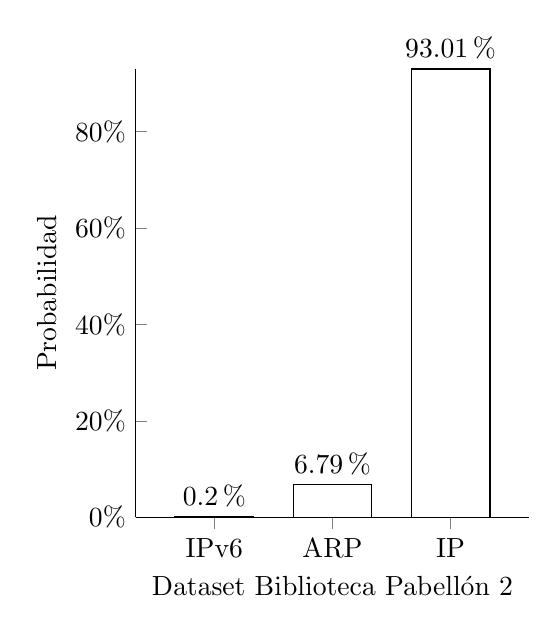
\begin{tikzpicture}
\begin{axis}[
    ybar,
    bar width=1cm, % Width of the bar
    x=1.5cm, % Distance between the centers of the bars
    enlarge x limits={abs=1cm}, % The distance between the center of the first bar and the left edge
    enlarge y limits=false,
    ymin=0,
    xtick=data,
    xlabel= {Dataset Biblioteca Pabellón 2},
    ylabel= {Probabilidad},
    symbolic x coords={IPv6,ARP,IP},
    point meta={y*100}, %y-Werte mal 100 für Prozent
    yticklabel={\pgfmathparse{\tick*100}\pgfmathprintnumber{\pgfmathresult}\%},
    axis lines*=left,
    clip=false
    ]
\addplot [
    draw=black,
    fill=white,
    nodes near coords={\pgfmathprintnumber{\pgfplotspointmeta}\,\%},
    error bars/.cd,
        y dir=both,
        y explicit
    ] coordinates{(IPv6,0.001998001998)
        (ARP,0.0679320679321)
        (IP,0.93006993007)};
\end{axis}
\end{tikzpicture}
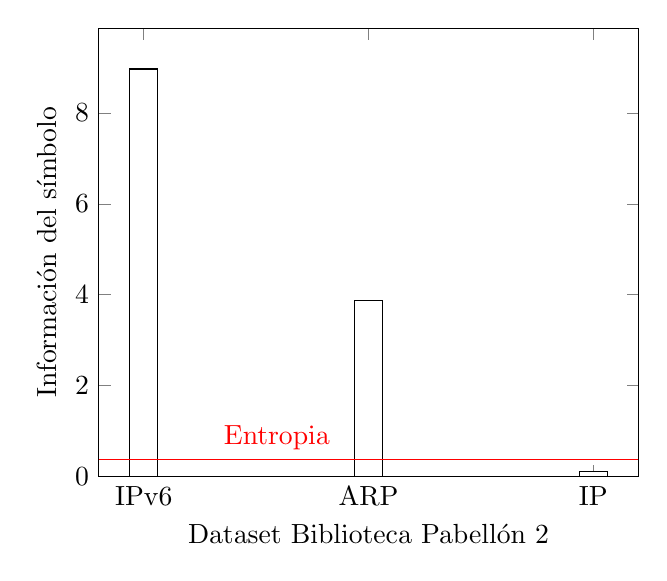
\begin{tikzpicture}
\begin{axis}[
    symbolic x coords={IPv6,ARP,IP},
        ylabel = {Información del símbolo},
        xlabel = {Dataset Biblioteca Pabellón 2},
        xtick=data,
        ymin=0]
    \addplot[ybar,fill=white] coordinates {
        (IPv6,8.9672262584)
        (ARP,3.8797634179)
        (IP,0.1045889014)
    };
    \draw [red] ({rel axis cs:0,0}|-{axis cs:ARP,0.378751880122}) -- ({rel axis cs:1,0}|-{axis cs:ARP,0.378751880122}) node [pos=0.33, above] {Entropia};
\end{axis}
\end{tikzpicture} \\

% Dataset 2 ----------------------------------

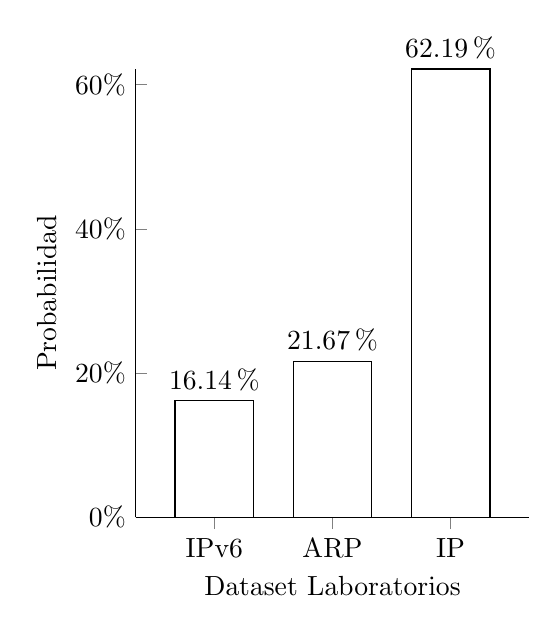
\begin{tikzpicture}
\begin{axis}[
    ybar,
    bar width=1cm, % Width of the bar
    x=1.5cm, % Distance between the centers of the bars
    enlarge x limits={abs=1cm}, % The distance between the center of the first bar and the left edge
    enlarge y limits=false,
    ymin=0,
    xtick=data,
    xlabel= {Dataset Laboratorios},
    ylabel= {Probabilidad},
    symbolic x coords={IPv6,ARP,IP},
    point meta={y*100}, %y-Werte mal 100 für Prozent
    yticklabel={\pgfmathparse{\tick*100}\pgfmathprintnumber{\pgfmathresult}\%},
    axis lines*=left,
    clip=false
    ]
\addplot [
    draw=black,
    fill=white,
    nodes near coords={\pgfmathprintnumber{\pgfplotspointmeta}\,\%},
    error bars/.cd,
        y dir=both,
        y explicit
    ] coordinates{
        (IPv6,0.161432269198)
        (ARP,0.216652286454)
        (IP,0.62191544434)};
\end{axis}
\end{tikzpicture}
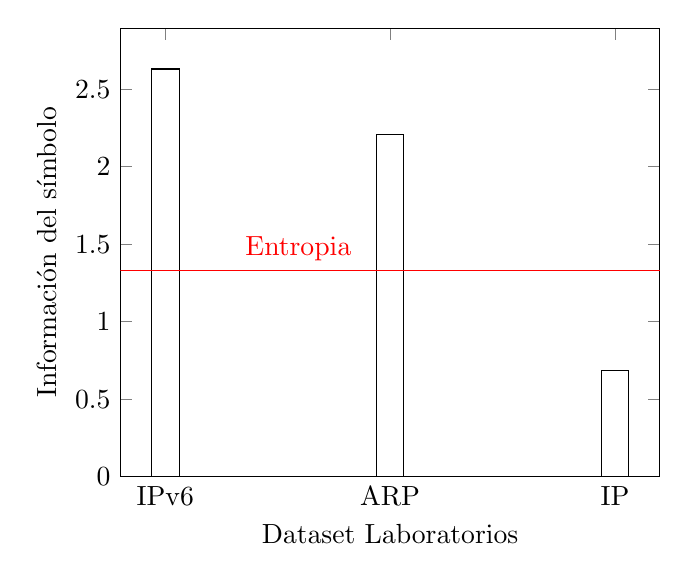
\begin{tikzpicture}
\begin{axis}[
    symbolic x coords={IPv6,ARP,IP},
        ylabel = {Información del símbolo},
        xlabel = {Dataset Laboratorios},
        xtick=data,
        ymin=0]
    \addplot[ybar,fill=white] coordinates {
        (IPv6,2.63099910265)
        (ARP,2.20654663262)
        (IP,0.6852096501)
    };
    \draw [red] ({rel axis cs:0,0}|-{axis cs:ARP,1.32892399253}) -- ({rel axis cs:1,0}|-{axis cs:ARP,1.32892399253}) node [pos=0.33, above] {Entropia};
\end{axis}
\end{tikzpicture} \\

% Dataset 3 ----------------------------------

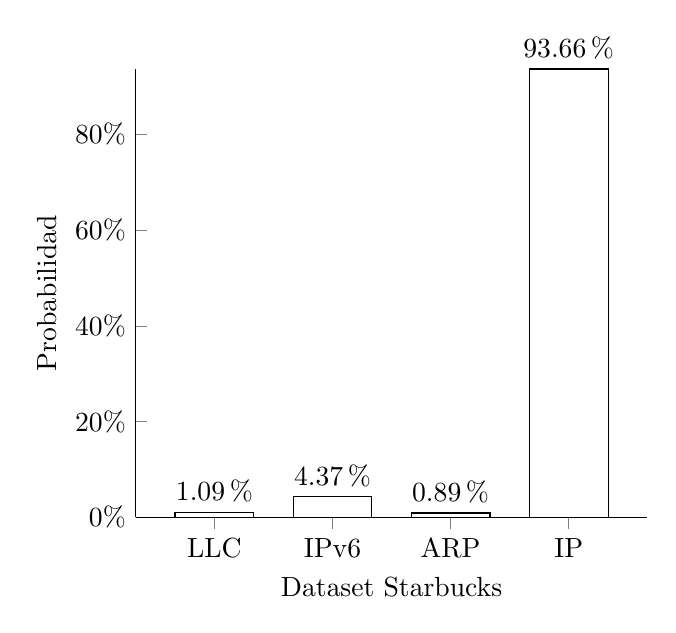
\begin{tikzpicture}
\begin{axis}[
    ybar,
    bar width=1cm, % Width of the bar
    x=1.5cm, % Distance between the centers of the bars
    enlarge x limits={abs=1cm}, % The distance between the center of the first bar and the left edge
    enlarge y limits=false,
    ymin=0,
    xtick=data,
    xlabel= {Dataset Starbucks},
    ylabel= {Probabilidad},
    symbolic x coords={LLC,IPv6,ARP,IP},
    point meta={y*100}, %y-Werte mal 100 für Prozent
    yticklabel={\pgfmathparse{\tick*100}\pgfmathprintnumber{\pgfmathresult}\%},
    axis lines*=left,
    clip=false
    ]
\addplot [
    draw=black,
    fill=white,
    nodes near coords={\pgfmathprintnumber{\pgfplotspointmeta}\,\%},
    error bars/.cd,
        y dir=both,
        y explicit
    ] coordinates{
        (LLC,0.0108909989989)
        (IPv6,0.0436853441738)
        (ARP,0.00885841701301)
        (IP,0.936565239814)};
\end{axis}
\end{tikzpicture}
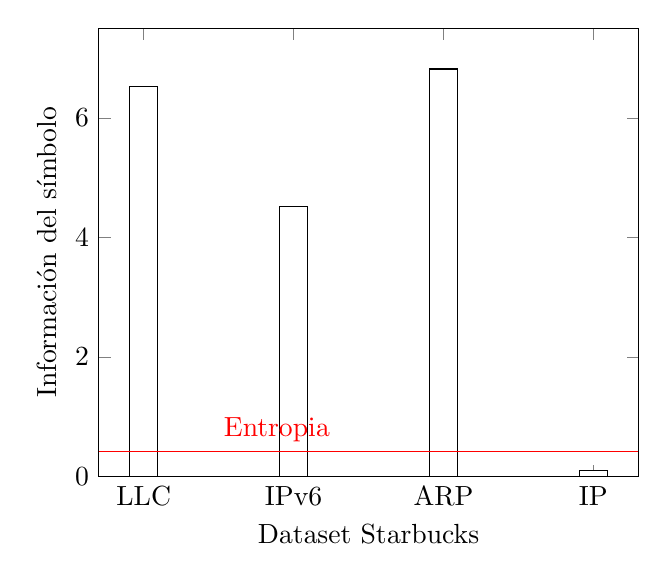
\begin{tikzpicture}
\begin{axis}[
    symbolic x coords={LLC,IPv6,ARP,IP},
        ylabel = {Información del símbolo},
        xlabel = {Dataset Starbucks},
        xtick=data,
        ymin=0]
    \addplot[ybar,fill=white] coordinates {
        (LLC,6.52071989553)
        (IPv6,4.51670683303)
        (ARP,6.81873537048)
        (IP,0.0945486008159)
        };
    \draw [red] ({rel axis cs:0,0}|-{axis cs:ARP,0.417285180797}) -- ({rel axis cs:1,0}|-{axis cs:ARP,0.417285180797}) node [pos=0.33, above] {Entropia};
\end{axis}
\end{tikzpicture} \\

% Dataset 4 ----------------------------------

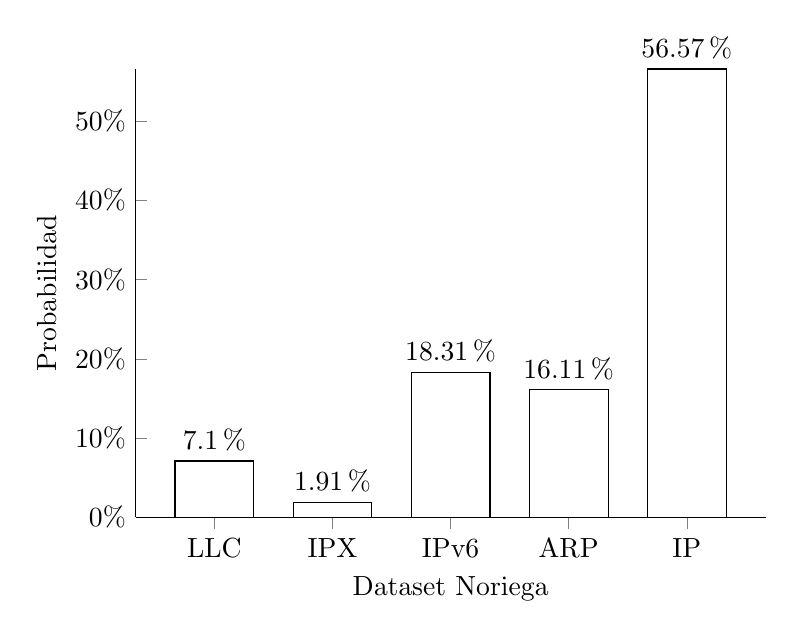
\begin{tikzpicture}
\begin{axis}[
    ybar,
    bar width=1cm, % Width of the bar
    x=1.5cm, % Distance between the centers of the bars
    enlarge x limits={abs=1cm}, % The distance between the center of the first bar and the left edge
    enlarge y limits=false,
    ymin=0,
    xtick=data,
    xlabel= {Dataset Noriega},
    ylabel= {Probabilidad},
    symbolic x coords={LLC,IPX,IPv6,ARP,IP},
    point meta={y*100}, %y-Werte mal 100 für Prozent
    yticklabel={\pgfmathparse{\tick*100}\pgfmathprintnumber{\pgfmathresult}\%},
    axis lines*=left,
    clip=false
    ]
\addplot [
    draw=black,
    fill=white,
    nodes near coords={\pgfmathprintnumber{\pgfplotspointmeta}\,\%},
    error bars/.cd,
        y dir=both,
        y explicit
    ] coordinates{
        (LLC,0.071005137663)
        (IPX,0.0191015676459)
        (IPv6,0.183111579502)
        (ARP,0.161111842972)
        (IP,0.565669872217)};
\end{axis}
\end{tikzpicture}
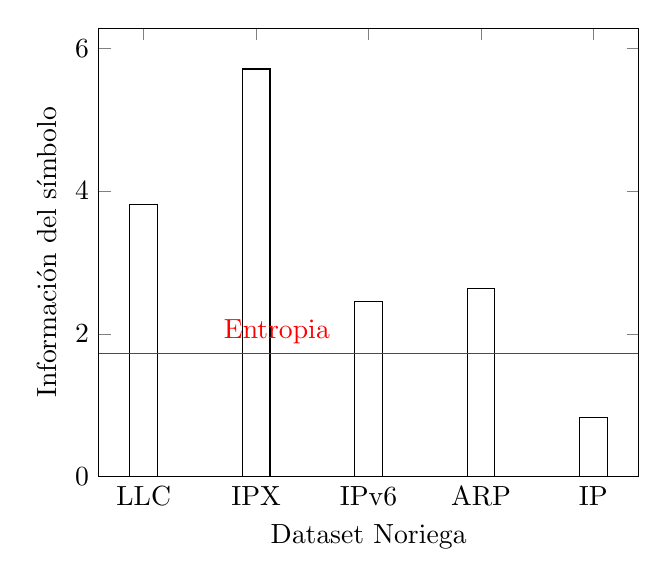
\begin{tikzpicture}
\begin{axis}[
    symbolic x coords={LLC,IPX,IPv6,ARP,IP},
        ylabel = {Información del símbolo},
        xlabel = {Dataset Noriega},
        xtick=data,
        ymin=0]
    \addplot[ybar,fill=white] coordinates {
        (LLC,3.81593277343)
        (IPX,5.71016514617)
        (IPv6,2.44920506857)
        (ARP,2.63386554765)
        (IP,0.821967760322)
    };
    \draw [red] ({rel axis cs:0,0}|-{axis cs:ARP,1.7178110768}) -- ({rel axis cs:1,0}|-{axis cs:ARP,1.7178110768}) node [pos=0.33, above] {Entropia};
\end{axis}
\end{tikzpicture} \\

% Discusion ------------------------------------

Por lo que podemos ver, la incidencia de \texttt{ARP} es muy baja en el primer Dataset ya que en una biblioteca hay poco recambio de dispositivos y pocos hosts, lo cual hace que la incidencia de \texttt{ARP} sea menor. En cambio, si hay muchos mas paquetes \texttt{IP}, lo cual tiene sentido porque es el protocolo que todos los hosts usan para conectarse a internet. Por su parte, IPv6 tiene menor incidencia que IP (y también ARP), se lo atribuimos a que esta versión de IP es menos usada. Entonces como podemos ver, el único símbolo predecible menor que la entropía es el de \texttt{IP}. 
%Es importante aclarar que en este Dataset observamos un comportamiento que en las demás capturas no sucedió: por cada paquete \texttt{ARP} "who-has" vemos inmediatamente otro \texttt{ARP} "is-at", lo cual sugiere una topología o funcionamiento distinto (sin embargo, todas las capturas fueron realizadas bajo las mismas condiciones).\\

En el segundo Dataset, ya podemos hablar de una red (el Laboratorio de Computación) en la cual no solamente hay muchos mas hosts, sino el recambio de dispositivos que entran y se van de la red es mayor, por lo cual la incidencia de \texttt{ARP} sube. A su vez, \texttt{IP} sigue siendo el protocolo más usado al igual que en el dataset anterior. \\

El tercer Dataset presenta un protocolo que no se veía en las capturas anteriores: LLC (Logic Link Control, que maneja el control de errores, control del flujo y entramado, entre otras cosas). LLC tiene menos incidencia que \texttt{IPv6} pero mas que \texttt{ARP}. Sin embargo hay una amplia mayoría de paquetes \texttt{IP}. \\

Analizando el cuarto Dataset (Noriega), vemos un nuevo protocolo: \texttt{IPX} (Internetworking Packet eXchange). De todos los datasets, este es el que menor incidencia \texttt{IP} tiene (56,57\%) sin embargo es mayor que la de los demás protocolos. \texttt{ARP} e \texttt{IPv6} comprenden entre el 15\% y 20\% de los paquetes cada uno. Así como vimos en el Dataset Laboratorios, esto se puede deber a la cantidad de gente que entra y sale de la red constantemente. \\

%Si tomamos la cantidad total de paquetes de cada protocolo en cada captura y la dividimos por el total de paquetes capturados, vemos la siguiente proporción: \\%

%\begin{center}
%    \begin{tikzpicture}
%        \pie[radius=5]{81/IP, 9/IPv6, 8/ARP, 1.7/LLC, 0.3/IPX}
%    \end{tikzpicture}
%\end{center}

% Finalmente, si definimos que un protocolo se distingue de otro según la cantidad total de paquetes de ese protocolo, el orden de distinsión es:

%\begin{enumerate}
%\item \texttt{IP}
%\item \texttt{IPv6}
%\item \texttt{ARP}
%\item \texttt{LLC}
%\item \texttt{IPX}
%\end{enumerate}

% end subsection

\subsection{Experimento incidencia de ARP}

Para poder observar la incidencia de paquetes \texttt{ARP} en la red, vamos a utilizar una serie de muestras tomadas de distintas redes y graficarlas en un histograma, 
después de mostrar los resultados daremos una explicación del por que de los mismo. Aclaración: todas las capturas son de 15 minutos.\\

Usamos dos datasets exlusivos para poder observar el comportamiento de redes más controladas, bajo la hipótesis de que entre más hosts hay más incidencia de paquetes ARP 
en la red. Los datasets que usamos son los siguientes:\\

\begin{itemize}
    \item \texttt{Dataset} Biblioteca pabellón 2 (wifi), captura de 15 minutos
    \item \texttt{Dataset} Laboratorios pabellón 1 (wifi), captura de 15 minutos
    \item \texttt{Dataset} Red de un Starbucks(wifi), captura de 15 minutos
    \item \texttt{Dataset} Red de la Biblioteca Noriega del pabellón 1(wifi), captura de 15 minutos
    \item \texttt{Dataset} Hogar de uno de los integrantes del grupo, sin ningun otro dispositivo(wifi), captura de 15 minutos
    \item \texttt{Dataset} Hogar de uno de los integrantes del grupo, con más dispositivos conectados a la red(wifi), captura de 15 minutos
\end{itemize}

\begin{figure}[H]
\centering
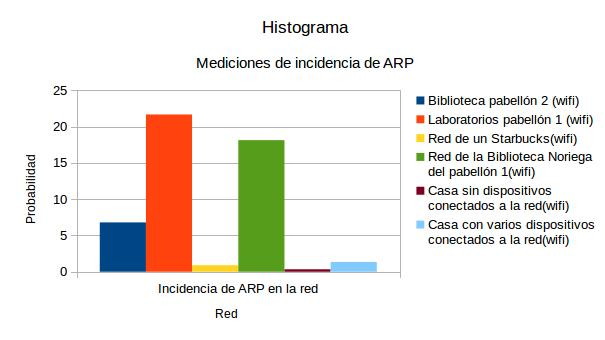
\includegraphics[width=150mm]{imagenes/IncidenciaARP.jpg}
\caption{Comparación de porcentaje de apariciones de ARP en distintas redes o con distintas condiciones.\label{overflow}}
\end{figure}

Como podemos ver, la red de los laboratorios tiene más porcentaje de paquetes \texttt{ARP} que el de la biblioteca. Esto se debe a que en el laboratorio del pabellón 1 ingresan
constantemente personas y, por lo tanto, la mayoría de ellos ingresan en la red a través de las computadoras del mismo o usando el wifi de estos con sus celulares. Esto
ocurre en menor medida en la biblioteca ya que no se usan computadoras que no sean propias de los que ingresan y, por lo tanto, hay mucho más tráfico de paquetes \texttt{ARP} en la red
de los laboratorios. Además al estar en una red privada, es más común que se efectúen envíos de mensajes entre computadoras y los routers de las mismas.\\

En menor medida tenemos los casos tomados en la red de un hogar, teniendo como sus dos mediciones a cuando solamente hay un dispositivo, el mismo con el que se realiza la medición,
conectado a la red y cuando hay más cantidad. Podemos ver que el tráfico de paquetes \texttt{ARP} es muy bajo en ambos casos en comparación a las muestras anteriores. Sin embargo,
cuando hay mayor cantidad de dispositivos el tráfico general aumenta y también el porcentaje de paquetes \texttt{ARP}, porque en este caso hay mas hosts.\\

Por último tenemos dos mediciones realizadas en la biblioteca Noriega y un Starbucks, en estas podemos ver resultados similares a los anteriores. La biblioteca tiene a muchas
gente entrando y saliendo, muchos de ellos se quedan a usar las instalaciones para estudiar con sus celulares y computadoras portátiles. En el Starbucks notamos que era menos
común cuando se realizo las mediciones.\\

La conclusión que podemos sacar es que, si bien estas muestras pertenecen a distintos lugares y horarios, podemos ver como el tráfico de paquetes \texttt{ARP} es más significativo cuando
la red tiende a recibir nuevos hosts con más constancia.

% end subsection


\subsection{Experimento nodos distinguidos}

Para distinguir los nodos de una red, tomaremos como fuente de información $S_1$ el campo
\texttt{IP} \textit{destino} de los paquetes \texttt{ARP Who-Has}.

No utilizaremos otros paquetes distintos de \texttt{ARP}, ya que queremos restringirnos a las comunicaciones internas de la subred. \\

Similar a como hicimos en el experimento de protocolos distinguidos, contamos la cantidad de apariciones de cada dirección \texttt{IP} en el campo destino de los paquetes \texttt{ARP Who-Has}, para luego calcular la probabilidad de aparición de cada \texttt{IP} en base a la cantidad total de paquetes capturados.

Usando esta probabilidad, calculamos la entropía y la comparamos con la información que aporta cada símbolo de $S_1$.\\

En este sentido, es interesante hacer notar que es muy probable que el Gateway de una red vaya a ser un nodo distinguido,
    ya que los otros nodos buscan enviarle información a su  \texttt{IP} constantemente.

\vspace{0.5em}


Los datasets utilizados en este experimento fueron: \\

\begin{itemize}
    \item Dataset Aulas DC (wifi), captura de 15 minutos
    \item Dataset Laboratorios DC (wifi), captura de 15 minutos
    \item Dataset Red de un Starbucks(wifi), captura de 15 minutos
    \item Dataset Red de la Biblioteca Noriega del pabellón 1(wifi), captura de 15 minutos
\end{itemize}

\vspace{0.5em}

A continuación mostramos los resultados para varios datasets. Se presentan:

\begin{itemize}
    \item Un grafo que permite visualizar la topología del dataset en cuestión. Los nodos en rojo son los distinguidos, es decir que su información es menor a la entropía de la fuente.
    \item La entropia.
    \item La cantidad de símbolos.
    \item Los nodos distinguidos.
\end{itemize}

\subsubsection{Aulas DC}

La topología de la red Aulas DC es la siguiente:

\begin{figure}[H]
    \centering
    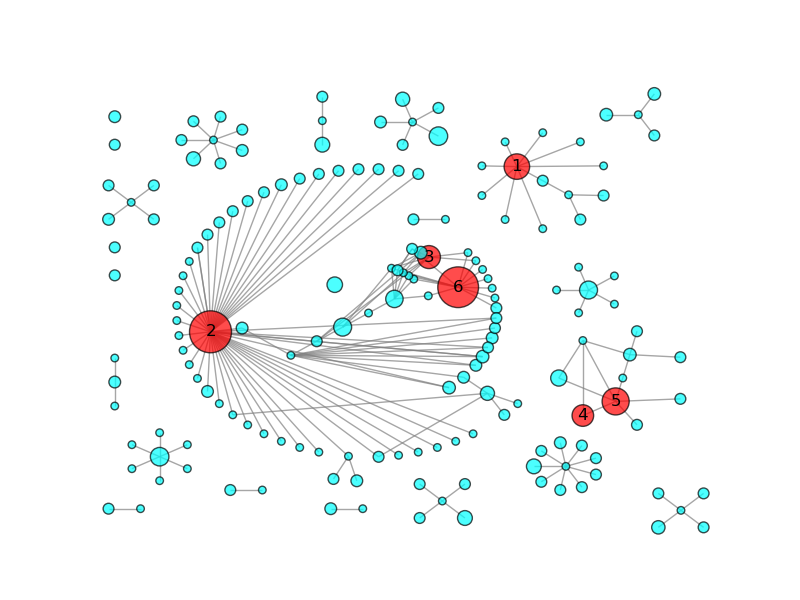
\includegraphics[width=0.85\textwidth]{imagenes/aulasDC.png}
    \caption{Topología de la red para el Dataset Aulas DC}
\end{figure}

La \textbf{entropia} de la fuente es: 4.98

La \textbf{cantidad símbolos} es: 101

Los \textbf{nodos distinguidos} son:

\begin{itemize}
    \item Con etiqueta 1: 10.2.6.250 tiene información 4.11
    \item Con etiqueta 2: 10.2.203.254 tiene información 2.53
    \item Con etiqueta 3: 10.2.2.205 tiene información 4.48
    \item Con etiqueta 4: 10.2.1.230 tiene información 4.70
    \item Con etiqueta 5: 10.2.1.254 tiene información 3.91
    \item Con etiqueta 6: 10.2.2.254 tiene información 2.62
\end{itemize}

En esta red encontramos la particularidad de que hay 2 nodos distinguidos que tienen
una cantidad de apariciones en la \texttt{IP} \textit{destino} muy parecida.
La \texttt{IP} 10.2.203.254 tiene 81 apariciones mientras que la \texttt{IP} 10.2.2.254 tiene 76 apariciones.

Además, nótese dichos nodos aparecen como dos componentes diferentes en el grafo que no hablan entre si,
lo que podría sugerir que la \texttt{IP} 10.2.203.254 es el \textit{Gateway} de la red
y la \texttt{IP} 10.2.2.254 podría ser un Switch.

\subsubsection{Laboratorios DC}

\begin{figure}[H]
    \centering
    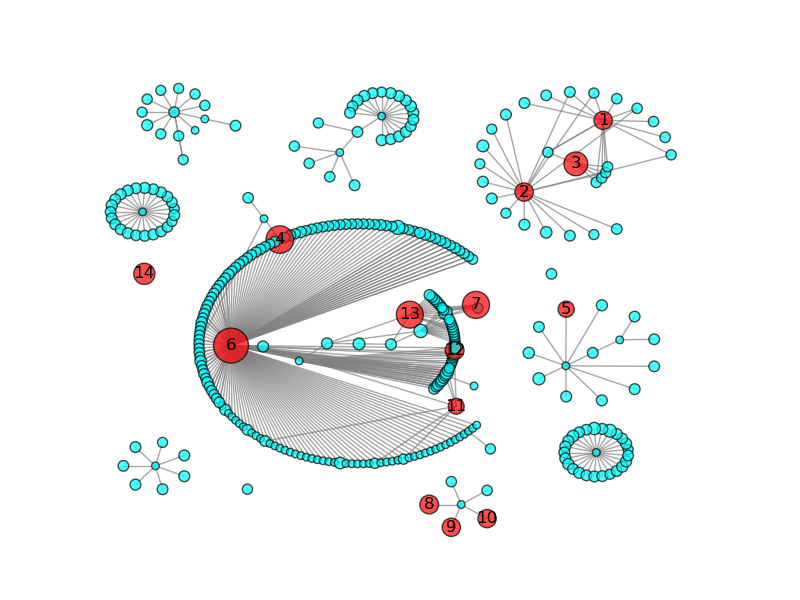
\includegraphics[width=0.85\textwidth]{imagenes/labosDC.png}
    \caption{Topología de la red para el Dataset Laboratorios DC}
\end{figure}

La \textbf{entropia} de la fuente es: 6.19

La \textbf{cantidad símbolos} es: 275

Los \textbf{nodos distinguidos} son:

\begin{itemize}
    \item Con etiqueta 1: 10.2.7.249 tiene información 5.34
    \item Con etiqueta 2: 10.2.7.254 tiene información 5.32
    \item Con etiqueta 3: 10.2.7.250 tiene información 4.35
    \item Con etiqueta 4: 10.2.203.27 tiene información 3.86
    \item Con etiqueta 5: 10.2.3.230 tiene información 5.86
    \item Con etiqueta 6: 10.2.203.254 tiene información 3.10
    \item Con etiqueta 7: 10.2.1.230 tiene información 3.91
    \item Con etiqueta 8: 10.2.0.67 tiene información 5.24
    \item Con etiqueta 9: 10.2.0.64 tiene información 5.34
    \item Con etiqueta 10: 10.2.0.65 tiene información 5.34
    \item Con etiqueta 11: 169.254.255.255 tiene información 5.95
    \item Con etiqueta 12: 169.254.231.139 tiene información 5.24
    \item Con etiqueta 13: 10.2.1.254 tiene información 3.94
    \item Con etiqueta 14: 10.2.0.187 tiene información 4.77
\end{itemize}

En esta red está claro que el \textit{Gateway} es la \texttt{IP} 10.2.203.254, debido a que
supera ampliamente a los demás nodos distinguidos.

Las particularidades a mencionar son:
\begin{itemize}
    \item La cantidad de nodos distinguidos es alta, lo cual lo atribuimos a la alta
        cantidad de \texttt{IPs} distintas.
        Dichos nodos asumimos que representan diferentes Switches en la red.
    \item Cabe destacar que el nodo distinguido con \texttt{IP} 10.2.0.187 (etiqueta 14)
        no se comunica con ningún otro nodo de la red. Al analizar los paquetes \texttt{ARP} que lo nombraban como
        destino, observamos que la fuente es la misma \texttt{IP}. No pudimos encontrar una explicación razonable para
        esto.
    \item Encontramos 2 nodos distinguidos (169.254.231.139 y 169.254.255.255) que no
        se encuentran en la subnet, lo cual tampoco pudimos explicar.
    \item Nos causó curiosidad ver que esta red tenía el mismo \textit{Gateway} que la red
        Aulas DC. Al investigar, vimos que ambas redes tenían el mismo DNS y dominio, por lo que suponemos
        que en el fondo son la misma red con dos nombres distintos.
\end{itemize}

\subsubsection{Biblioteca Noriega}

\begin{figure}[H]
    \centering
    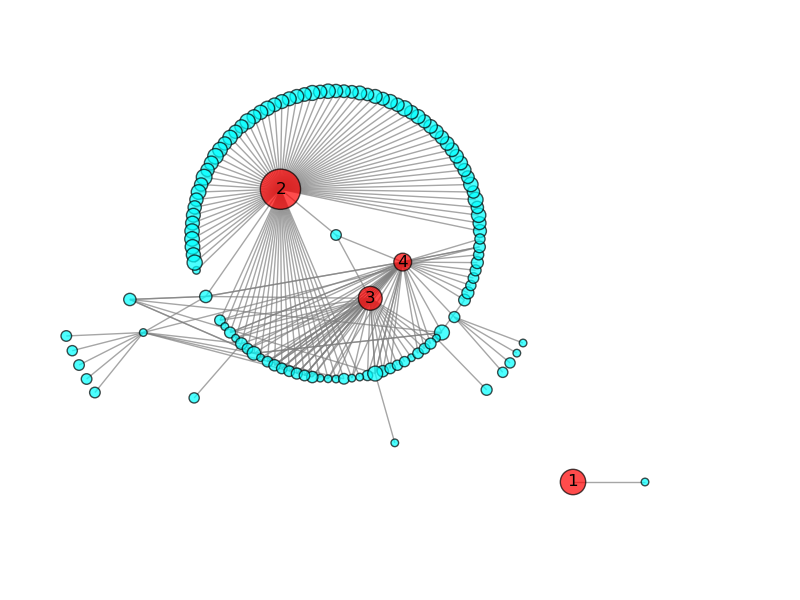
\includegraphics[width=0.85\textwidth]{imagenes/noriega.png}
    \caption{Topología de la red para el Dataset Biblioteca Noriega}
\end{figure}

La \textbf{entropía} de la fuente es: 5.91

La \textbf{cantidad símbolos} es: 110

Los \textbf{nodos distinguidos} son:

\begin{itemize}
    \item Con etiqueta 1: 10.255.255.254 tiene información 4.13
    \item Con etiqueta 2: 157.92.15.199 tiene información 2.66
    \item Con etiqueta 3: 157.92.15.133 tiene información 4.35
    \item Con etiqueta 4: 157.92.15.136 tiene información 5.45
\end{itemize}

En esta red está claro que el \textit{Gateway} es la \texttt{IP} 157.92.15.199, debido a que
supera ampliamente a los demás nodos distinguidos.

Las particularidades a mencionar son:
\begin{itemize}
    \item Los nodos con etiqueta 3 y 4 (157.92.15.133 y 157.92.15.136) suponemos
        que son Switches que particionan la red, evitando conflictos.
    \item  Se vuelve a presentar el caso de una \texttt{IP} que está fuera de la red: 10.255.255.254, que tiene la particularidad de estar muy aislado de los otros nodos.
\end{itemize}



\subsubsection{Starbucks}

\begin{figure}[H]
    \centering
    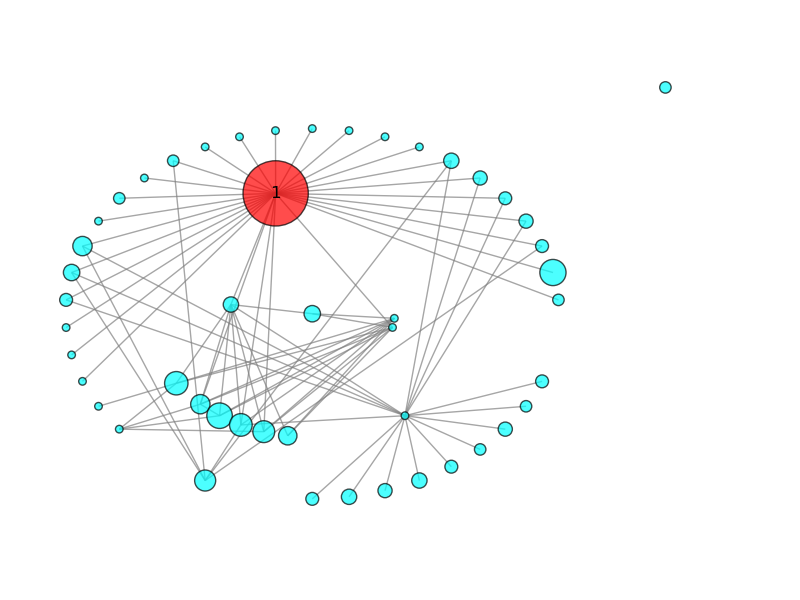
\includegraphics[width=0.85\textwidth]{imagenes/starbucks.png}
    \caption{Topología de la red para el Dataset Starbucks}
\end{figure}

La \textbf{entropía} de la fuente es: 3.51

La \textbf{cantidad símbolos} es: 32

Los \textbf{nodos distinguidos} son:

\begin{itemize}
    \item Con etiqueta 1: 10.254.70.1 tiene información 1.21
\end{itemize}

En esta red está claro que el \textit{Gateway} es la \texttt{IP} 10.254.70.1, debido a que
es el único nodo distinguido.
